\begin{sidewaysfigure}
	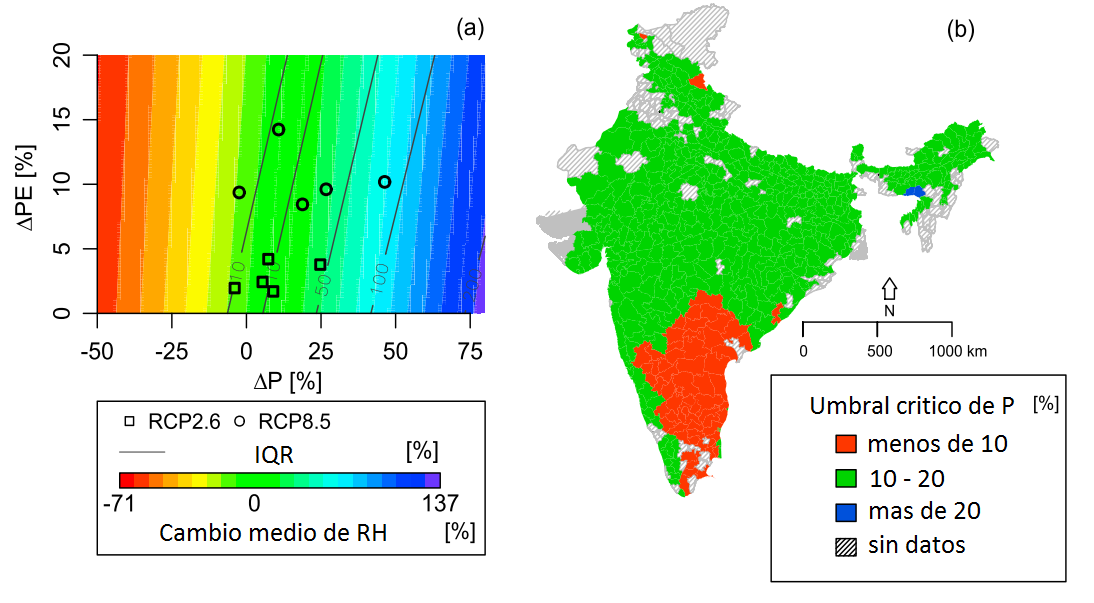
\includegraphics[scale=0.75]{Images/Singh02.png}
	\centering
	\caption{a) Vulnerabilidad de los RH a escala de la India estimada en función del cambio de precipitación ($\Delta P$) y evapotranspiración potencial ($\Delta PE$). Colores y lineas grises representan la mediana y el IQR del índice de vulnerabilidad. respectivamente. Adicionalmente se muestra (puntos y cuadrados) las proyecciones de $P$ y $PE$ de los modelos de cambio climático (CMIP-5). b) Variación espacial del cambio critico de $P$ que resulta en una reducción de 25\% de la disponibilidad RH en la India.}
	{\raggedright FUENTE: \citet{Singh2015}. \par}
	\label{fig:Singh02}
	
	\thisfloatpagestyle{empty}
\end{sidewaysfigure}
